\documentclass[../Master.tex]{subfiles}
\begin{document}

For an action schema $A$, $\mathbb{P}_A$ is the set of all predicates in the domain that can be applied with the arguments of $A$.
\[
    \mathbb{P}_A = \left\{
        p \left( x_1, \dots, x_{|p|} \right)
        \; | \; \left\{ x_1, \dots, x_{|p|} \right\} \subseteq params(A)
    \right\}
\]

\begin{figure}
    \centering
    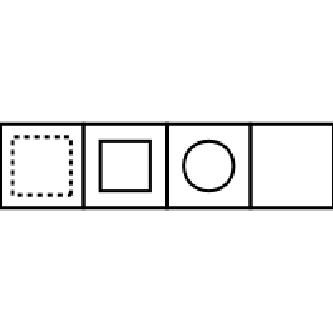
\includegraphics[scale=0.7]{../Graphics/sokoSmall}
    \caption{\label{fig:sokoSmall} Sokoban state with only one applicable \texttt{move-h} action. The tiles are named $t_1 \dots t_4$, from left to right. The crate object is named $c$.}
\end{figure}

We will now consider the problem of learning the preconditions of an action schema $A$.

In \cite{Walsh2008}, the authors suggest maintaining a set of all possible conjunctions of $k$ or less predicates (where $k$ is the maximal number of predicates allowed in action schema preconditions), and --- on action failure --- marking the conjunctions predicting that the action would have succeeded as disproven.

We propose a solution where individual predicates are proven and disproven to be preconditions based on the following observations:
\begin{itemize}
    \item When $a$ succeeds, there are predicates which, if they had been preconditions, would have caused failure. These can be immediately disproven to be preconditions.
    \item When $a$ fails, there are a number of predicates which could be responsible for the failure if they are preconditions. Although it is indeterminable which of them are preconditions and which are not, this information can be saved and analysed later, when more information is available.
\end{itemize}

In the following we will analyse how the aforementioned predicate sets can be deduced from a single state transition, and later discuss how knowledge obtained from earlier state transitions can be used to prove predicates to be preconditions.

As a running example, we will once again use the sokoban domain, where the environment starts in the following state (visualized in figure \ref{fig:sokoSmall}):
\begin{equation*}
    s_0 =
    \left\{
        \begin{gathered}
            \texttt{sokobanAt}(t_3), \texttt{at}(b, t_2), \texttt{goal}(t_1), \\
            \texttt{clear}(t_1), \texttt{clear}(t_4), \\
            \texttt{hAdj}(t_1, t_2), \texttt{hAdj}(t_2, t_3),
            \texttt{hAdj}(t_3, t_4), \\
            \texttt{hAdj}(t_2, t_1), \texttt{hAdj}(t_3, t_2),
            \texttt{hAdj}(t_4, t_3)
        \end{gathered}
    \right\}
\end{equation*}

From this state, we will analyse the outcomes of different applications of the \texttt{move-h} action, whose preconditions are reprinted below:

\begin{align*}
    P_{\texttt{move-h}}^+ &= \left\{
        \texttt{sokobanAt}(from), \texttt{clear}(to), \texttt{hAdj}(from, to)
        \right\} \\
    P_{\texttt{move-h}}^- &= \emptyset
\end{align*}

As can be seen, there is only one applicaple \texttt{move-h} action in state $s_0$, namely $\texttt{move-h}(t_3,t_4)$. As the agent is unaware of this fact, it may apply other $\texttt{move-h}$ actions, which will all fail. The only information available to it is that both the positive and negative preconditions are subsets of $\mathbb{P}_{\texttt{move-h}}$, since no other predicate can be a precondition due to the scoping rule.

\begin{equation*}
\mathbb{P}_{\texttt{move-h}} =
\left\{
    \begin{gathered}
        \texttt{sokobanAt}(to), \texttt{sokobanAt}(from), \\
        \texttt{clear}(to), \texttt{clear}(from), \\
        \texttt{goal}(to), \texttt{goal}(from), \\
        \texttt{vAdj}(from, to), \texttt{vAdj}(to, from), \\
        \texttt{vAdj}(from, from), \texttt{vAdj}(to, to), \\
        \texttt{hAdj}(from, to), \texttt{hAdj}(to, from), \\
        \texttt{hAdj}(from, from), \texttt{hAdj}(to, to), \\
        \texttt{at}(from, to), \texttt{at}(to, from)
    \end{gathered}
\right\}
\end{equation*}


\subsubsection*{Action success}
Since the action was successfully applied, $s$ satisfied all preconditions, meaning that
        \[ g\left[P^+\right] \subseteq s_t \land
            g\left[P^-\right] \subseteq \mathbb{P} \setminus s_t
        \]
It follows trivially that any predicate $p \in \mathbb{P}$ for which $g(p) \notin s_t$ can not be a positive precondition, as that would have caused the action to fail. Similarly, if $g(p) \in s_t$, then $p$ can not be a negative precondition. Since these predicates can be immediately disproven,

\begin{equation} \label{eq:DPlusTrans}
    D^+ = \left\{ x \; | \; x \in \mathbb{P} \land g(x) \notin s \right\}
\end{equation}

\begin{equation} \label{eq:DMinusTrans}
    D^- = \left\{ x \; | \; x \in \mathbb{P} \land g(x) \in s \right\}
\end{equation}

Hence, the sets of potential positive and negative preconditions can be enumerated by \eqref{eq:UPlusTrans} and \eqref{eq:UMinusTrans}, respectively.

\begin{equation} \label{eq:UPlusTrans}
    U^+ = \mathbb{P} \setminus D^+ =
        \left\{ x \; | \; x \in \mathbb{P} \land g(x) \in s_t \right\}
\end{equation}
\begin{equation} \label{eq:UMinusTrans}
    U^- = \mathbb{P} \setminus D^- =
        \left\{ x \; | \; x \in \mathbb{P} \land g(x) \notin s_t \right\}
\end{equation}

Note that it is unknown whether any of these predicates are actually preconditions, but it is certain that $P^+ \subseteq U^+$ and $P^- \subseteq U^-$.

\begin{example}[\texttt{move-h} action succeeded] \label{ex:moveSucceeded}
In case the sokoban agent applies the action $\texttt{move-h}(t_3, t_4)$ in state $s_0$, the resulting state $s_1$ will have the visible effect that the sokoban relocated from $t_3$ to $t_4$. \eqref{eq:DPlusTrans} and \eqref{eq:DMinusTrans} can now be applied to $s_0$ to obtain the following:

\begin{equation*}
    D^+ = \left\{
        \begin{gathered}
            \texttt{sokobanAt}(to), \texttt{clear}(from), \\
            \texttt{vAdj}(from, to), \texttt{vAdj}(to, from), \\
            \texttt{vAdj}(from, from), \texttt{vAdj}(to, to), \\
            \texttt{hAdj}(from, from), \texttt{hAdj}(to, to), \\
            \texttt{at}(from, to), \texttt{at}(to, from), \\
            \texttt{goal}(from), \texttt{goal}(to)
        \end{gathered}
    \right\}
\end{equation*}

\begin{equation*}
    D^- = \left\{
        \begin{gathered}
            \texttt{sokobanAt}(from), \texttt{clear}(to), \\
            \texttt{hAdj}(from, to), \texttt{hAdj}(to, from)
        \end{gathered}
    \right\}
\end{equation*}

\noindent\rule{\textwidth}{1pt}
\end{example}

\subsubsection*{Action failure}
In case of action failure, at least one of $A$'s preconditions were not satisfied by $s$, but there is no indication from the environment on which predicate(s) violated a precondition by their presence in or absence from $s$. However, it is certain that either a negative precondition was violated by a predicate $p \in s$, or a positive precondition was violated by a predicate absent from $s$. The predicates that would have caused the failure if part of $P^+$ (resp. $P^-$) are called the positive (resp. negative) candidates and are denoted $c^+$ (resp. $c^-$):

\begin{equation} \label{eq:cPlus}
    c^+ = \left\{ x \; | \; x \in \mathbb{P} \land g(x) \notin s \right\}
\end{equation}
\begin{equation} \label{eq:cMinus}
    c^- = \left\{ x \; | \; x \in \mathbb{P} \land g(x) \in s \right\}
\end{equation}

Since the action failed, it holds trivially that \textit{some} predicates in $c^+$ or $c^-$ (or both) are preconditions, ie.

\begin{equation} \label{eq:inv}
    \left| c^+ \cap P^+ \right| + \left| c^- \cap P^- \right| \geq 1
\end{equation}

This is an important invariant; if the sets $c^+$ and $c^-$ can be reduced such that only one predicate remain in $c^+ \cup c^-$ while \eqref{eq:inv} is maintained, then that predicate is proven to be a precondition (negative or positive, depending on whether it was a member of $c^+$ or $c^-$) <Does this need to be proven?>. Formally,
\begin{theorem} \label{th:precondProof}
    If \eqref{eq:inv} holds for $c^+$ and $c^-$, then it holds that
    \begin{itemize}
        \item If $c^+ = \{p\} \land c^- = \emptyset$ then $p$ is a positive precondition ($p \in P^+$).
        \item If $c^- = \emptyset \land c^- = \{p\}$ then $p$ is a negative precondition ($p \in P^-$).
    \end{itemize}
\end{theorem}

It is clear that if a predicate is disproven to be a precondition, then it can not be the precondition that was violated by $s$, and caused the action to fail. As such, it can safely be disregarded as a candidate.

\begin{theorem} \label{th:invHolds}
    If \eqref{eq:inv} holds for candidate sets $c^+$ and $c^-$, and a predicate $p$ has been disproven to be a positive or negative precondition, then \eqref{eq:inv} holds for $c^+ \setminus \{ p \}$ and $c^- \setminus \{ p \}$.
\end{theorem}

\begin{example}[\texttt{move-h} action failed]
    If the agent decides to move one tile to the left in state $s_0$, and appropriately executes the \texttt{move-h}$(t_3, t_2)$ action, it will discover that the new state is exactly the same as the old, and that the action therefore must have failed. The ungrounded predicates that could have caused the failure are then the following:
    \begin{equation*}
        c^+ = \left\{
            \begin{gathered}
                \texttt{sokobanAt}(to), \\
                \texttt{clear}(to), \texttt{clear}(from), \\
                \texttt{goal}(to), \texttt{goal}(from), \\
                \texttt{vAdj}(from, to), \texttt{vAdj}(to, from), \\
                \texttt{vAdj}(from, from), \texttt{vAdj}(to, to), \\
                \texttt{hAdj}(from, from), \texttt{hAdj}(to, to), \\
                \texttt{at}(from, to), \texttt{at}(to, from)
            \end{gathered}
        \right\}
    \end{equation*}

    \begin{equation*}
        c^- = \left\{
            \begin{gathered}
                \texttt{sokobanAt}(from), \\
                \texttt{hAdj}(from, to), \texttt{hAdj}(to, from)
            \end{gathered}
        \right\}
    \end{equation*}

    Out of these, only \texttt{clear}$(to)$ is a precondition. If the agent has available the knowledge from Example \ref{ex:moveSucceeded}, it can remove $D^+$ from the positive candidates and $D^-$ from the negatives, while --- according to theorem \ref{th:invHolds} --- maintaining invariant \eqref{eq:inv}, yielding

    \begin{equation*}
        \left( c^+ \setminus D^+, c^- \setminus D^- \right) =
        \left( \{\texttt{clear}(to) \}, \emptyset \right)
    \end{equation*}

    Of all the predicates that could have caused $\texttt{move-h}(t_3, t_2)$ to fail if they had been preconditions, $\texttt{clear}(to)$ is the only one that has not been disproven to be one. Therefore, it must have been what caused the failure, and is proven to be a precondition.

    \noindent\rule{\textwidth}{1pt}
\end{example}

However, if a predicate $p \in c^+ \cup c^-$ is \textit{proven} to be a precondition, then its removal could violate \eqref{eq:inv}: If $p$ is the only predicate in $c^+ \cup c^-$ that is a precondition, (such that $c^+ \cap P^+ \cup c^- \cap P^- = \{ p \}$), then
\begin{equation*}
    \left| c^+ \cap P^+ \right| + \left| c^- \cap c^+ \right| = 0
\end{equation*}

As a consequence, if $c^+ \cup c^-$ contains more than one precondition, ie. if

\begin{equation*}
    \left| c^+ \cap P^+ \right| + \left| c^- \cap P^- \right| > 1,
\end{equation*}

then $\left( c^+, c^- \right)$ can never be reduced to a singleton set without violating \eqref{eq:inv}. Furthermore, a candidate set containing a predicate proven to be a precondition can never yield more knowledge: If $p$ is retained in $c$, then one of the following cases apply:
\begin{itemize}
    \item $\left(c^{+}\cap P^{+}\right)\cup\left(c^{-}\cap P^{-}\right)=\{ p \}$, ie. $p$ is the only predicate in $c$ that is a precondition. Then $c$ could eventually be reduced to the singleton set $\{ p \}$, which does not produce any new knowledge, since $p$ is already known to be a precondition.

    \item $\left|\left(c^{+}\cap P^{+}\right)\cup\left(c^{-}\cap P^{-}\right)\right|>1$, ie. more than two predicates in $c$ are preconditions of $A$. As mentioned above, $c$ can never be reduced to the singleton set, and no knowledge can be gained from it.
\end{itemize}
In both cases, retaining the set $c$ as it is will not provide any new knowledge. Thus, a candidate set can be discarded when one of its members are proven to be present in $P^{\pm}$.

\begin{example}[\texttt{move-h} action failed]
    If the agent tries to execute the action $\texttt{move-h}(t_3, t_1)$, it will once again find that the application was unsuccessful, since it is required that the destination tile is horizontally adjacent to the source tile. In this case, the set of positive candidates $c^+$ will contain both $\texttt{hAdj}(from, to)$ and $\texttt{hAdj}(to, from)$. Since these are not in $D^+$ (from example \ref{ex:moveSucceeded}), the candidates can not be reduced to a singleton set. Furthermore, because of the symmetry of the two predicates, the one will never appear in a state without the other, and if one of them is absent from a state, so is the other. Although $P^+$ only contains $\texttt{hAdj}(to, from)$, $\texttt{hAdj}(from, to)$ is an implicit precondition; if is violated in a state, so is $\texttt{hAdj}(from, to)$.

    A consequence of this is that when the adjacency precondition is violated, the candidate set will always contain at least two preconditions, and can as such never be reduced to a singleton set.

    \noindent\rule{\textwidth}{1pt}
\end{example}

\subsection*{Using prior knowledge}

We will now present an algorithm (see algorithm \ref{algo:precondLearn}) for obtaining knowledge about preconditions from a series of state transitions. The algorithm takes as input a state transition $(s, a, s')$ as well as prior knowledge about the action schema for $a$, consisting of the following:

\begin{itemize}
    \item Sets $K^+$ and $K^-$, containing the ungrounded predicates that have previously been proven to be positive and negative preconditions, respectively.
    \item Sets $D^+$ and $D^-$, containing the ungrounded predicates that have previously been proven to \textit{not} be positive and negative preconditions, respectively.
    \item A set $C$ containing candidate sets of the form $\left(c^+, c^- \right)$, where each candidate set satisfies the invariant in \eqref{eq:inv}.
\end{itemize}

On action success, the sets of predicates that can be disproven to be preconditions based on this transition is calculated using \eqref{eq:DPlusTrans} and \eqref{eq:DMinusTrans}, and added to the existing knowledge:

\begin{equation*}
    D_t^+ = D_{t-1}^+ \cup \left\{ x \; | \; x \in \mathbb{P} \land g(x) \notin s_t \right\}
\end{equation*}

\begin{equation*}
    D_t^- = D_{t-1}^- \cup \left\{ x \; | \; x \in \mathbb{P} \land g(x) \in s_t \right\}
\end{equation*}

On action failure, the candidate sets are determined using \eqref{eq:cPlus} and \eqref{eq:cMinus}, and are added to the set $C$.

It now holds that either more predicates have been disproven, or one more candidate set have been added to $C$. According to theorem \ref{th:invHolds}, each candidate set in $C$ can now be reduced by removing disproven predicates, while maintaining invariant \eqref{eq:inv}:
\begin{equation} \label{reduceCands}
    C = \left\{ \left( x^+ \setminus D^+, c^- \setminus D^- \right)
            \; | \; \left( x^+, x^- \right) \in C
        \right\}
\end{equation}

By theorem \ref{th:precondProof}, members of any singleton candidate set can now be added to the proven knowledge:

\begin{equation} \label{eq:extractKnown}
    K^{\pm} = \left\{
        x^{\pm} \; | \; \left( x^+, x^- \right) \in C \land
        \left| x^{\pm} \right| = 1 \land
        \left|  x^+ \right| + \left| x^- \right| = 1
    \right\}
    \cup K^{\pm}
\end{equation}

As discussed previously, any candidate set containing a predicate which have already been proven to be a precondition can be safely removed from $C$, as no more knowledge can be obtained from it, formally:

\begin{equation} \label{eq:removeKnown}
    C = \left\{
        \left( x^+, x^- \right) \; | \;
        \left( x^+, x^- \right) \in C \land
        \left(
            x^+ \cap K^+ \neq \emptyset \lor x^- \cap K^- \neq \emptyset
        \right)
    \right\}
\end{equation}

\begin{algorithm}
    \caption{Algorithm for learning preconditions}
    \label{algo:precondLearn}

    \begin{algorithmic}
        \Function {$\textsc{Precond-learn}$} {$\left( s, a, s'\right), K^\pm$, $U^\pm$, $C$}
            \If {$s' \neq s$}
                \State $c^+ \gets
                    \left\{ x \; | \; x \in \mathbb{P} \land g(x) \notin s_t \right\}$
                \State $c^- \gets
                    \left\{ x \; | \; x \in \mathbb{P} \land g(x) \in s_t \right\}$
                \State $C \gets C \cup \left\{ \left( c^+, c^- \right) \right\}$
            \ElsIf {$s' = s$}
                \State $D^+ \gets D^+ \cup
                    \left\{
                        x \; | \; x \in \mathbb{P} \land g(x) \notin s_t
                    \right\}$
                \State $D^- \gets D^- \cup
                    \left\{
                        x \; | \; x \in \mathbb{P} \land g(x) \in s_t
                    \right\}$
            \EndIf
            \State Remove disproven predicates from candidates
            \Comment \emph{see \eqref{reduceCands}}
            \State $K^\pm \gets \left\{ \textnormal{singleton sets from } C\right\}$ $\cup K^\pm$
            \Comment \emph{see \eqref{eq:extractKnown}}
            \State Remove candidate sets from $C$ which contain a predicate in $K^\pm$
            \Comment \emph{see \eqref{eq:removeKnown}}
            \State \Return $(K^\pm, D^\pm, C)$
        \EndFunction
    \end{algorithmic}
\end{algorithm}

\end{document}
